\section{AI Workload Profiling}

\label{sec:ai-workloads}

\subsection{Conservation AI Workloads}

Zoo Network's AI workloads differ from typical blockchain transactions:

\begin{table}[t]
\centering
\begin{tabular}{lccc}
\toprule
\textbf{Workload} & \textbf{Gas/Call} & \textbf{Compute Intensity} & \textbf{State Access} \\
\midrule
Species classification & 500K & High (CNN forward pass) & Low \\
Habitat suitability & 350K & Medium (gradient boosting) & Medium \\
Population model & 800K & High (Monte Carlo sim) & Low \\
Encrypted inference & 1.2M & Very High (FHE + CNN) & Low \\
Gradient aggregation & 210K & Medium (vector addition) & High \\
\bottomrule
\end{tabular}
\caption{Conservation AI workload characteristics on Zoo EVM.}
\label{tab:ai-workloads}
\end{table}

\subsection{GPU Efficiency by Workload}

AI workloads achieve significantly higher GPU efficiency than financial transactions because they are compute-bound rather than memory-bound:

\begin{figure}[t]
\centering
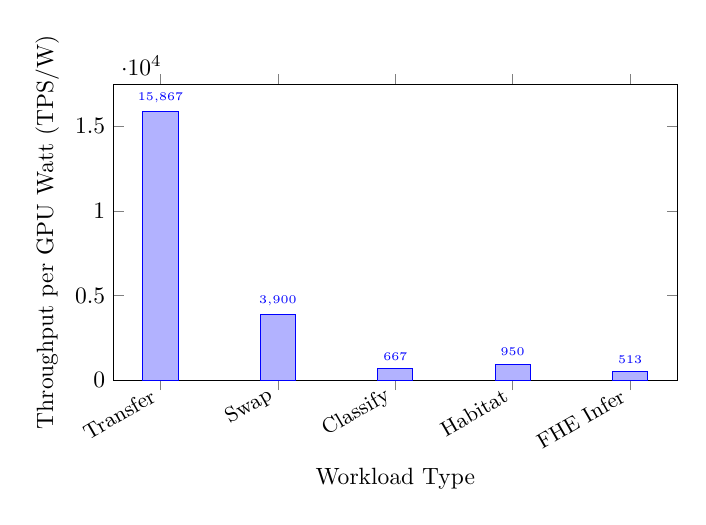
\begin{tikzpicture}[scale=0.85]
    \begin{axis}[
        ybar,
        xlabel={Workload Type},
        ylabel={Throughput per GPU Watt (TPS/W)},
        symbolic x coords={Transfer, Swap, Classify, Habitat, FHE Infer},
        xtick=data,
        xticklabel style={rotate=30, anchor=east, font=\small},
        ymin=0,
        bar width=15pt,
        width=10cm,
        height=6cm,
        nodes near coords,
        nodes near coords style={font=\tiny}
    ]
    \addplot coordinates {
        (Transfer, 15867) (Swap, 3900) (Classify, 667) (Habitat, 950) (FHE Infer, 513)
    };
    \end{axis}
\end{tikzpicture}
\caption{Energy efficiency (TPS per GPU Watt) by workload type. AI workloads have lower TPS but higher computational value per transaction.}
\label{fig:efficiency}
\end{figure}

\subsection{Opcode Heat Map}

The most frequently executed opcodes differ between financial and AI workloads:

\begin{table}[t]
\centering
\begin{tabular}{lcc}
\toprule
\textbf{Opcode} & \textbf{DeFi (\%)} & \textbf{AI (\%)} \\
\midrule
\texttt{ADD/SUB} & 18\% & 31\% \\
\texttt{MUL/DIV} & 8\% & 24\% \\
\texttt{SLOAD/SSTORE} & 22\% & 6\% \\
\texttt{CALL/STATICCALL} & 15\% & 8\% \\
\texttt{KECCAK256} & 12\% & 3\% \\
Precompile calls & 3\% & 22\% \\
Other & 22\% & 6\% \\
\bottomrule
\end{tabular}
\caption{Opcode frequency distribution for DeFi vs AI workloads. AI workloads are arithmetic-heavy with frequent precompile calls.}
\label{tab:opcodes}
\end{table}

